% ============================================================================
% CHAPTER 1F: CHEMICAL SYSTEMS
% ============================================================================

\section{Chemical Systems}
\label{sec:chemical}

Chemical processes involve mass and energy balances coupled with reaction kinetics. These systems often exhibit nonlinear behavior, time delays, and complex interactions, making them challenging but important control applications.

% ============================================================================
\subsection{Continuous Stirred-Tank Reactor (CSTR)}
\label{subsec:cstr}
% ============================================================================

The CSTR is a fundamental unit in chemical engineering and a classic control problem.

\begin{figure}[htbp]
\centering
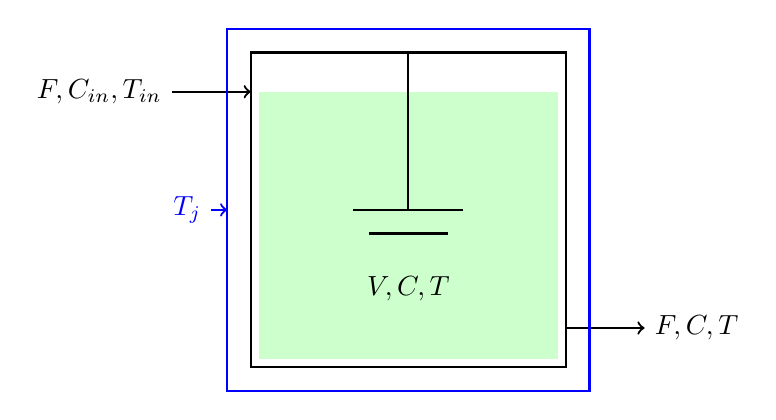
\begin{tikzpicture}
    % Tank
    \draw[thick] (0,0) -- (0,4) -- (4,4) -- (4,0) -- cycle;

    % Liquid
    \fill[green!20] (0.1,0.1) rectangle (3.9,3.5);

    % Stirrer
    \draw[thick] (2,4) -- (2,2);
    \draw[thick] (1.3,2) -- (2.7,2);
    \draw[thick] (1.5,1.7) -- (2.5,1.7);

    % Inlet
    \draw[->, thick] (-1,3.5) -- (0,3.5) node[left, pos=0] {$F, C_{\text{in}}, T_{\text{in}}$};

    % Outlet
    \draw[->, thick] (4,0.5) -- (5,0.5) node[right] {$F, C, T$};

    % Jacket
    \draw[thick, blue] (-0.3,-0.3) rectangle (4.3,4.3);
    \draw[->, thick, blue] (-0.5,2) -- (-0.3,2) node[left, pos=0] {$T_j$};

    % Labels
    \node at (2,1) {$V, C, T$};
\end{tikzpicture}
\caption{Continuous stirred-tank reactor with cooling jacket.}
\label{fig:cstr}
\end{figure}

\subsubsection{Assumptions}

\begin{itemize}
    \item Perfect mixing (uniform concentration and temperature)
    \item Constant volume $V$ and density $\rho$
    \item Constant flow rate $F$ (in = out)
    \item Single first-order irreversible reaction: $A \to B$
\end{itemize}

\subsubsection{Component Mass Balance}

\begin{equation}
V\frac{\dd C_A}{\dd t} = F(C_{A,\text{in}} - C_A) - Vk(T)C_A
\end{equation}

where $k(T)$ is the temperature-dependent reaction rate constant.

\subsubsection{Arrhenius Equation}

\begin{equation}
k(T) = k_0 \exp\left(-\frac{E_a}{RT}\right)
\end{equation}

where:
\begin{itemize}
    \item $k_0$ = pre-exponential factor (1/s)
    \item $E_a$ = activation energy (J/mol)
    \item $R$ = universal gas constant (8.314 J/mol$\cdot$K)
\end{itemize}

\subsubsection{Energy Balance}

\begin{equation}
\rho V C_p\frac{\dd T}{\dd t} = F\rho C_p(T_{\text{in}} - T) + (-\Delta H_r)Vk(T)C_A - UA(T - T_j)
\end{equation}

where:
\begin{itemize}
    \item $\Delta H_r$ = heat of reaction (J/mol, negative for exothermic)
    \item $UA$ = heat transfer coefficient times area (W/K)
    \item $T_j$ = jacket temperature (K)
\end{itemize}

\subsubsection{Linearized Model}

Linearizing about steady-state $(C_{A0}, T_0)$:
\begin{align}
\frac{\dd \Delta C_A}{\dd t} &= a_{11}\Delta C_A + a_{12}\Delta T + b_1\Delta C_{A,\text{in}} \\
\frac{\dd \Delta T}{\dd t} &= a_{21}\Delta C_A + a_{22}\Delta T + b_2\Delta T_j
\end{align}

State-space form:
\begin{equation}
\begin{bmatrix} \Delta\dot{C}_A \\ \Delta\dot{T} \end{bmatrix} = \mA \begin{bmatrix} \Delta C_A \\ \Delta T \end{bmatrix} + \mB \begin{bmatrix} \Delta C_{A,\text{in}} \\ \Delta T_j \end{bmatrix}
\end{equation}

\begin{examplebox}[title=Example 1.12: CSTR Linearization]
A CSTR operates at steady-state with:
\begin{itemize}
    \item $V = 1$ m$^3$, $F = 0.1$ m$^3$/min
    \item $C_{A0} = 2$ mol/L, $T_0 = 350$ K
    \item $k_0 = 10^{10}$ min$^{-1}$, $E_a/R = 8750$ K
\end{itemize}

The linearized $\mA$ matrix elements are:
\begin{align}
a_{11} &= -\frac{F}{V} - k(T_0) = -0.1 - k_0\ee^{-8750/350} = -0.1 - 1.2 = -1.3 \text{ min}^{-1} \\
a_{12} &= -C_{A0}\frac{\dd k}{\dd T}\bigg|_{T_0} = -C_{A0}k(T_0)\frac{E_a}{RT_0^2} = -0.17 \text{ mol/L$\cdot$K$\cdot$min}
\end{align}

The negative $a_{12}$ indicates that increased temperature increases reaction rate, consuming more $C_A$.
\end{examplebox}

% ============================================================================
\subsection{Mixing Tank}
\label{subsec:mixing}
% ============================================================================

\begin{figure}[htbp]
\centering
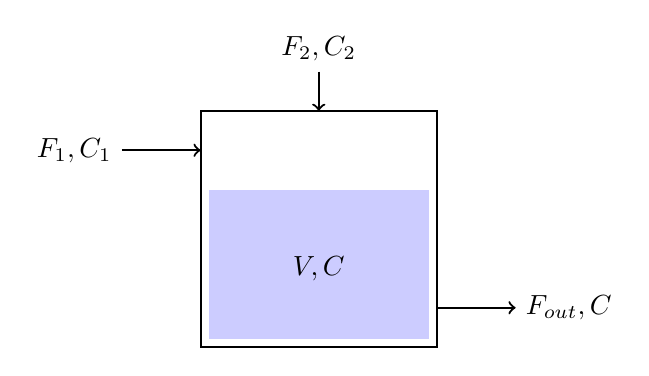
\begin{tikzpicture}
    % Tank
    \draw[thick] (0,0) -- (0,3) -- (3,3) -- (3,0) -- cycle;
    \fill[blue!20] (0.1,0.1) rectangle (2.9,2);

    % Inlet 1
    \draw[->, thick] (-1,2.5) -- (0,2.5) node[left, pos=0] {$F_1, C_1$};

    % Inlet 2
    \draw[->, thick] (1.5,3.5) -- (1.5,3) node[above, pos=0] {$F_2, C_2$};

    % Outlet
    \draw[->, thick] (3,0.5) -- (4,0.5) node[right] {$F_{\text{out}}, C$};

    % Labels
    \node at (1.5,1) {$V, C$};
\end{tikzpicture}
\caption{Mixing tank with two inlets.}
\label{fig:mixing_tank}
\end{figure}

\subsubsection{Mass Balance (Total)}

\begin{equation}
\frac{\dd(\rho V)}{\dd t} = \rho_1 F_1 + \rho_2 F_2 - \rho F_{\text{out}}
\end{equation}

For constant density and volume: $F_{\text{out}} = F_1 + F_2$

\subsubsection{Component Balance}

\begin{equation}
V\frac{\dd C}{\dd t} = F_1 C_1 + F_2 C_2 - (F_1 + F_2)C
\end{equation}

Transfer function (for constant $F_1$, $F_2$):
\begin{equation}
\frac{C(s)}{C_1(s)} = \frac{F_1/V}{s + (F_1+F_2)/V} = \frac{F_1/(F_1+F_2)}{\tau s + 1}
\end{equation}

where $\tau = V/(F_1 + F_2)$ is the residence time.

% ============================================================================
\subsection{pH Neutralization}
\label{subsec:ph}
% ============================================================================

pH control is notoriously difficult due to the highly nonlinear relationship between acid/base concentration and pH.

\begin{equation}
\text{pH} = -\log_{10}[H^+]
\end{equation}

For a strong acid-strong base system:
\begin{equation}
[H^+] = \frac{C_a - C_b + \sqrt{(C_a - C_b)^2 + 4K_w}}{2}
\end{equation}

where $K_w = 10^{-14}$ at 25°C.

\textbf{Titration curve:} The pH changes dramatically near the equivalence point, creating a high-gain nonlinearity.

\begin{figure}[htbp]
\centering
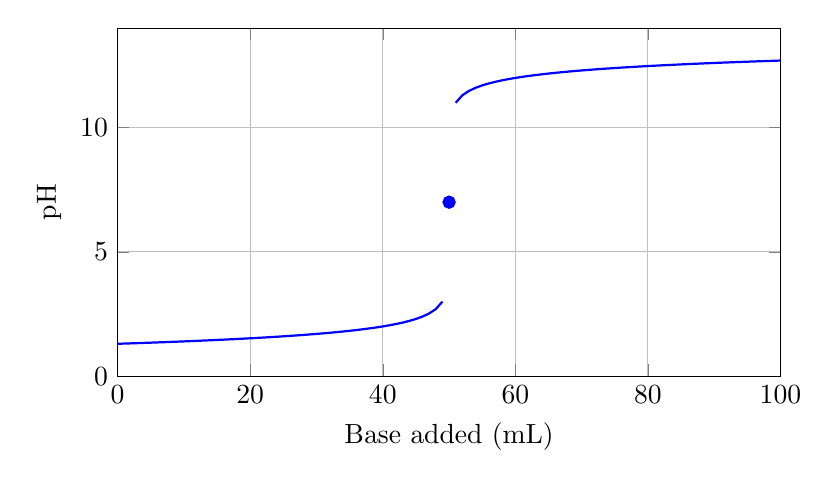
\begin{tikzpicture}
\begin{axis}[
    width=10cm, height=6cm,
    xlabel={Base added (mL)},
    ylabel={pH},
    xmin=0, xmax=100,
    ymin=0, ymax=14,
    grid=major
]
\addplot[blue, thick, domain=0:49, samples=50] {-log10(0.1*(50-x)/100)};
\addplot[blue, thick, domain=51:100, samples=50] {14 + log10(0.1*(x-50)/100)};
\addplot[blue, thick, mark=*] coordinates {(50,7)};
\end{axis}
\end{tikzpicture}
\caption{Typical pH titration curve showing high gain near equivalence.}
\label{fig:ph_titration}
\end{figure}

% ============================================================================
\subsection{Distillation Column}
\label{subsec:distillation}
% ============================================================================

Distillation separates mixtures based on volatility differences.

\begin{figure}[htbp]
\centering
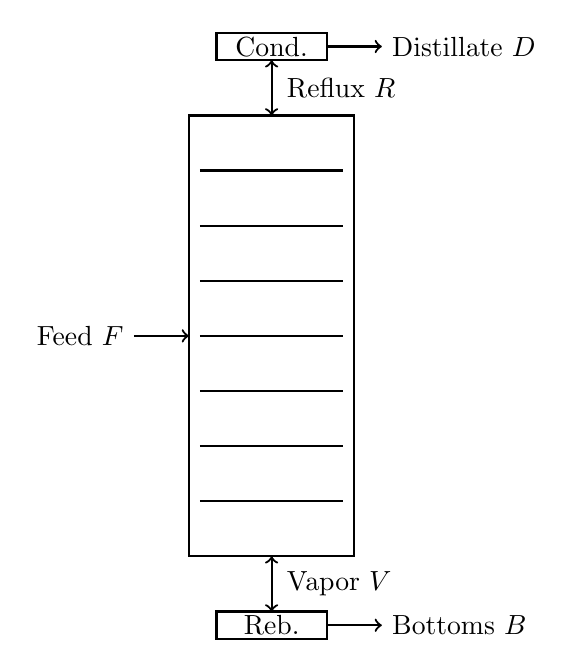
\begin{tikzpicture}[scale=0.7]
    % Column
    \draw[thick] (0,0) -- (0,8) -- (3,8) -- (3,0) -- cycle;

    % Trays
    \foreach \y in {1,2,...,7} {
        \draw[thick] (0.2,\y) -- (2.8,\y);
    }

    % Feed
    \draw[->, thick] (-1,4) -- (0,4) node[left, pos=0] {Feed $F$};

    % Overhead
    \draw[->, thick] (1.5,8) -- (1.5,9);
    \draw[thick] (0.5,9) rectangle (2.5,9.5);
    \node at (1.5,9.25) {Cond.};
    \draw[->, thick] (2.5,9.25) -- (3.5,9.25) node[right] {Distillate $D$};
    \draw[->, thick] (1.5,9) -- (1.5,8);
    \node[right] at (1.6,8.5) {Reflux $R$};

    % Bottom
    \draw[->, thick] (1.5,0) -- (1.5,-1);
    \draw[thick] (0.5,-1.5) rectangle (2.5,-1);
    \node at (1.5,-1.25) {Reb.};
    \draw[->, thick] (2.5,-1.25) -- (3.5,-1.25) node[right] {Bottoms $B$};
    \draw[->, thick] (1.5,-1) -- (1.5,0);
    \node[right] at (1.6,-0.5) {Vapor $V$};
\end{tikzpicture}
\caption{Distillation column schematic.}
\label{fig:distillation}
\end{figure}

\subsubsection{Simplified Model}

For a binary mixture, the composition dynamics on tray $n$:
\begin{equation}
M_n\frac{\dd x_n}{\dd t} = L_{n-1}x_{n-1} + V_{n+1}y_{n+1} - L_n x_n - V_n y_n
\end{equation}

where:
\begin{itemize}
    \item $M_n$ = liquid holdup on tray
    \item $L_n$ = liquid flow rate
    \item $V_n$ = vapor flow rate
    \item $x_n$ = liquid composition (mole fraction)
    \item $y_n$ = vapor composition
\end{itemize}

Vapor-liquid equilibrium:
\begin{equation}
y_n = \frac{\alpha x_n}{1 + (\alpha - 1)x_n}
\end{equation}

where $\alpha$ is the relative volatility.

% ============================================================================
\subsection{Batch Reactor}
\label{subsec:batch}
% ============================================================================

Unlike continuous reactors, batch reactors have no flow during reaction:

\begin{align}
\frac{\dd C_A}{\dd t} &= -k(T)C_A \\
\frac{\dd T}{\dd t} &= \frac{(-\Delta H_r)k(T)C_A}{\rho C_p} - \frac{UA(T - T_j)}{\rho V C_p}
\end{align}

The concentration decreases exponentially (for first-order kinetics):
\begin{equation}
C_A(t) = C_{A0}\exp\left(-\int_0^t k(T(\tau))\,\dd\tau\right)
\end{equation}

% ============================================================================
\subsection{Reaction Kinetics}
\label{subsec:kinetics}
% ============================================================================

\subsubsection{Zero-Order Reaction}

\begin{equation}
\frac{\dd C}{\dd t} = -k
\end{equation}

Solution: $C(t) = C_0 - kt$

\subsubsection{First-Order Reaction}

\begin{equation}
\frac{\dd C}{\dd t} = -kC
\end{equation}

Solution: $C(t) = C_0\ee^{-kt}$

Half-life: $t_{1/2} = \ln(2)/k$

\subsubsection{Second-Order Reaction}

\begin{equation}
\frac{\dd C}{\dd t} = -kC^2
\end{equation}

Solution: $\frac{1}{C(t)} = \frac{1}{C_0} + kt$

\subsubsection{Enzyme Kinetics (Michaelis-Menten)}

\begin{equation}
\frac{\dd C}{\dd t} = -\frac{V_{\max}C}{K_m + C}
\end{equation}

where $V_{\max}$ is maximum rate and $K_m$ is the Michaelis constant.

% ============================================================================
\subsection{Process Dead Time}
\label{subsec:dead_time}
% ============================================================================

Many chemical processes exhibit significant time delays (dead time, transport lag):

\begin{equation}
y(t) = u(t - \theta)
\end{equation}

Transfer function:
\begin{equation}
G(s) = \ee^{-\theta s}
\end{equation}

Dead time makes control more challenging. Common approximations:

\textbf{First-order Padé:}
\begin{equation}
\ee^{-\theta s} \approx \frac{1 - \theta s/2}{1 + \theta s/2}
\end{equation}

\textbf{Second-order Padé:}
\begin{equation}
\ee^{-\theta s} \approx \frac{1 - \theta s/2 + (\theta s)^2/12}{1 + \theta s/2 + (\theta s)^2/12}
\end{equation}

\begin{examplebox}[title=Example 1.13: First-Order Plus Dead Time (FOPDT)]
Many chemical processes can be approximated as:
\begin{equation}
G(s) = \frac{K\ee^{-\theta s}}{\tau s + 1}
\end{equation}

For a heat exchanger with $K = 2$ °C/\%, $\tau = 60$ s, $\theta = 10$ s:
\begin{equation}
G(s) = \frac{2\ee^{-10s}}{60s + 1}
\end{equation}

The dead-time-to-time-constant ratio $\theta/\tau = 10/60 = 0.17$ indicates this system is relatively easy to control.
\end{examplebox}

% ============================================================================
\subsection{CSTR Schematic and Inlet/Outlet Configuration}
\label{subsec:cstr_schematic_detailed}
% ============================================================================

\begin{figure}[htbp]
\centering
\begin{tikzpicture}[scale=0.95]
    % Reactor vessel (square cross-section with sharp corners)
    \draw[thick, UofSCBlack] (1,0) -- (1,5) -- (5,5) -- (5,0) -- cycle;
    \fill[UofSCAtlantic!12] (1.2,0.2) rectangle (4.8,4);

    % Stirrer motor
    \draw[thick, UofSCBlack] (3,5.2) circle (0.25);
    \node at (3,5.2) {\tiny M};

    % Stirrer shaft and impeller
    \draw[thick, UofSCBlack] (3,5) -- (3,3);
    \draw[thick, UofSCCongaree] (2.3,3) -- (3.7,3);
    \draw[thick, UofSCCongaree] (2.5,2.5) -- (3.5,2.5);

    % Liquid region
    \fill[UofSCAtlantic!25] (1.2,0.2) rectangle (4.8,3.8);

    % Inlet port
    \draw[thick, UofSCBlack] (0.3,3.5) -- (1,3.5);
    \draw[thick, UofSCHoneycomb, fill=UofSCHoneycomb!40] (0.5,3.3) rectangle (0.8,3.7);
    \draw[->, thick, UofSCGarnet] (-0.2,3.5) -- (0.3,3.5);
    \node[left, small, UofSCGarnet] at (-0.3,3.5) {$F_{\text{in}}$};

    % Inlet concentration and temperature labels
    \node[left, small, UofSCBlack] at (-0.1,3.2) {$C_{A,\text{in}}$};
    \node[left, small, UofSCBlack] at (-0.1,2.9) {$T_{\text{in}}$};

    % Outlet port (bottom)
    \draw[thick, UofSCBlack] (3,0) -- (3,-0.8);
    \draw[thick, UofSCHoneycomb, fill=UofSCHoneycomb!40] (2.8,-0.5) rectangle (3.2,-0.1);
    \draw[->, thick, UofSCGarnet] (3,-0.8) -- (3,-1.5);
    \node[below, small, UofSCGarnet] at (3,-1.6) {$F_{\text{out}}$};

    % Outlet concentration and temperature labels
    \node[right, small, UofSCBlack] at (3.3,-0.3) {$C_A$};
    \node[right, small, UofSCBlack] at (3.3,-0.6) {$T$};

    % Cooling jacket
    \draw[thick, UofSCRose, dash pattern=on 3pt off 2pt] (0.7,-0.2) rectangle (5.3,5.3);
    \draw[->, thick, UofSCRose] (0.4,2.5) -- (0.7,2.5);
    \node[left, small, UofSCRose] at (0.2,2.5) {$T_j$};

    % Reactor content label
    \node[align=center, small] at (3,2) {$V, C_A, T$\\$\rho, C_p$};

    % Reaction indicator
    \node[align=center, small, UofSCCongaree] at (3,0.8) {$A \to B$\\$k(T)$};

    % Legend box
    \draw[thick, UofSCAtlantic] (5.8,0.5) rectangle (8.8,3.5);
    \node[anchor=west, small] at (6,3.2) {\textbf{Variables:}};
    \node[anchor=west, small] at (6,2.8) {$F$ = volumetric flow};
    \node[anchor=west, small] at (6,2.4) {$C_A$ = concentration};
    \node[anchor=west, small] at (6,2.0) {$T$ = temperature};
    \node[anchor=west, small] at (6,1.6) {$V$ = reactor volume};
    \node[anchor=west, small] at (6,1.2) {$k(T)$ = reaction rate};
    \node[anchor=west, small] at (6,0.8) {constant};
\end{tikzpicture}
\caption{Continuous stirred-tank reactor (CSTR) with detailed inlet/outlet ports, cooling jacket, and labeled flows showing reactant concentration and temperature at inlet and outlet.}
\label{fig:cstr_detailed_schematic}
\end{figure}

The inlet provides fresh reactant at concentration $C_{A,\text{in}}$ and temperature $T_{\text{in}}$, while the outlet removes mixture at the reactor conditions $(C_A, T)$ since perfect mixing is assumed. The cooling jacket maintains temperature control through $T_j$.

% ============================================================================
\subsection{Reaction Rate vs. Temperature: Arrhenius Behavior}
\label{subsec:reaction_rate_temperature}
% ============================================================================

\begin{figure}[htbp]
\centering
\begin{tikzpicture}
\begin{axis}[
    width=10cm,
    height=7cm,
    xlabel={Temperature (K)},
    ylabel={Reaction Rate Constant $k(T)$ (min$^{-1}$)},
    xmin=250, xmax=450,
    ymin=0, ymax=8,
    grid=major,
    grid style={gray!20},
    xlabel style={font=\small},
    ylabel style={font=\small},
    tick label style={font=\small}
]

% Arrhenius curve: k(T) = k0 * exp(-Ea/RT)
% k0 = 1e10 min^-1, Ea/R = 8750 K
\addplot[
    UofSCGarnet,
    thick,
    smooth,
    domain=250:450,
    samples=100
] {1e-8 * exp(-8750/x)};

% Mark key operating points
\addplot[
    only marks,
    mark=*,
    mark size=5pt,
    UofSCAtlantic
] coordinates {(300,0.05) (350,0.5) (400,3.5)};

% Annotations for operating points
\node[UofSCAtlantic, anchor=south] at (axis cs:300,0.05) {$T_1=300\text{ K}$};
\node[UofSCAtlantic, anchor=south] at (axis cs:350,0.5) {$T_{\text{nom}}=350\text{ K}$};
\node[UofSCAtlantic, anchor=south] at (axis cs:400,3.5) {$T_2=400\text{ K}$};

\end{axis}

% Temperature sensitivity region highlight (outside axis)
\draw[UofSCHorseshoe!30, fill=UofSCHorseshoe!15] (4.2,1.5) rectangle (5.2,5.5);
\node[UofSCHorseshoe, font=\small] at (4.7,5.3) {Sensitive};
\node[UofSCHorseshoe, font=\small] at (4.7,5.0) {Region};

% Add equation box
\draw[thick, UofSCCongaree] (0.3,6.5) rectangle (2.8,7.8);
\node[anchor=west, UofSCCongaree, small] at (0.4,7.5) {$k(T) = k_0 \exp\left(-\frac{E_a}{RT}\right)$};
\node[anchor=west, small] at (0.4,7.1) {$k_0 = 10^{10}$ min$^{-1}$};
\node[anchor=west, small] at (0.4,6.7) {$E_a/R = 8750$ K};

\end{tikzpicture}
\caption{Arrhenius equation showing exponential increase in reaction rate with temperature. The nonlinear relationship creates control challenges, with the system becoming increasingly sensitive to temperature in the operating range.}
\label{fig:arrhenius_curve}
\end{figure}

The exponential dependence means small temperature changes can dramatically affect reaction rate. For a 50 K increase from 350 K to 400 K, the reaction rate increases approximately 7-fold. This nonlinear behavior is fundamental to exothermic reaction dynamics and runaway concerns.

% ============================================================================
\subsection{Exercises: Chemical Systems}
% ============================================================================

\begin{exercise}
A CSTR with volume 500 L and flow rate 50 L/min processes a first-order reaction with $k = 0.1$ min$^{-1}$. Feed concentration is 2 mol/L.
\begin{enumerate}[label=(\alph*)]
    \item Find the steady-state exit concentration
    \item Find the residence time
    \item Write the transfer function from $C_{\text{in}}$ to $C$
    \item Find the time constant
\end{enumerate}
\end{exercise}

\begin{exercise}
A mixing tank blends two streams: Stream 1 at 100 L/min with 10\% salt, and Stream 2 at 50 L/min with 2\% salt. Tank volume is 1000 L.
\begin{enumerate}[label=(\alph*)]
    \item Find the steady-state exit concentration
    \item If Stream 1 concentration suddenly changes to 15\%, find the new steady-state and the time to reach 90\% of the change
\end{enumerate}
\end{exercise}

\begin{exercise}
An exothermic batch reactor starts at 25°C with 1000 mol of reactant. Heat of reaction is $-50$ kJ/mol, heat capacity is 4 kJ/kg$\cdot$K, mass is 1000 kg, and reaction rate constant is $k = 0.01$ min$^{-1}$ at 25°C with $E_a/R = 5000$ K.
\begin{enumerate}[label=(\alph*)]
    \item Write the coupled ODEs for concentration and temperature (adiabatic case)
    \item Estimate the adiabatic temperature rise if reaction goes to completion
\end{enumerate}
\end{exercise}

\begin{exercise}
\textbf{CSTR Reaction Kinetics:} A CSTR operates with a second-order reaction $2A \to B$ having rate law $r = kC_A^2$ with $k = 0.1$ L/(mol$\cdot$min). The reactor volume is 100 L and inlet concentration is 1 mol/L.
\begin{enumerate}[label=(\alph*)]
    \item For inlet flow 10 L/min, calculate the steady-state concentration
    \item If temperature increases causing $k$ to double, find the new steady-state
    \item Compare reaction rates at both operating points
\end{enumerate}
\end{exercise}

\begin{exercise}
\textbf{CSTR Temperature Control:} An exothermic reaction in a CSTR generates heat at rate $\dot{Q}_{\text{gen}} = (-\Delta H_r)k(T)C_A \cdot V$ where $-\Delta H_r = 50$ kJ/mol, $k(T)$ follows Arrhenius with $E_a/R = 8750$ K. The cooling jacket removes heat at $\dot{Q}_{\text{cool}} = UA(T - T_j)$ with $UA = 5$ kW/K.
\begin{enumerate}[label=(\alph*)]
    \item Write the energy balance ODE
    \item For $T_j = 350$ K (set at nominal operating point), find the steady-state temperature
    \item If $T_j$ suddenly drops to 300 K, predict the qualitative response
\end{enumerate}
\end{exercise}

\begin{exercise}
A process has FOPDT model with $K = 1.5$, $\tau = 120$ s, and $\theta = 30$ s.
\begin{enumerate}[label=(\alph*)]
    \item Write the transfer function
    \item Calculate $\theta/\tau$ and comment on controllability
    \item Use first-order Padé approximation and find the system poles
\end{enumerate}
\end{exercise}

\begin{exercise}
\textbf{pH Control Challenge:} A strong acid-strong base neutralization uses $[H^+] = \frac{C_a - C_b + \sqrt{(C_a - C_b)^2 + 4K_w}}{2}$ where $K_w = 10^{-14}$.
\begin{enumerate}[label=(\alph*)]
    \item With acid concentration 0.1 M flowing at 100 mL/min and base 0.1 M at 95 mL/min, find pH at steady-state
    \item Calculate the sensitivity $\frac{d(\text{pH})}{dC_b}$ at this point
    \item If base flow increases to 100.5 mL/min, estimate the new pH and explain the control difficulty
\end{enumerate}
\end{exercise}
